\begin{figure}[htbp]
	\centering
	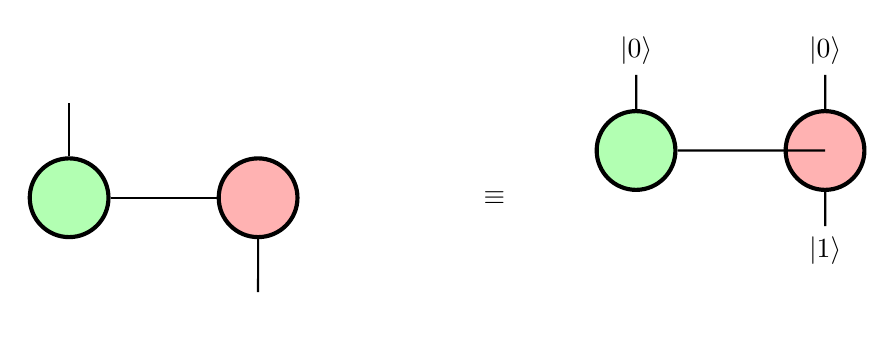
\begin{tikzpicture}[scale=1.2]
		\node[draw, circle, fill=green!30, minimum size=1cm, line width=1.5pt] (g1) at (0,0) {};
		\draw[thick] (g1) -- (0,1) node[above] {};
		\draw[thick] (g1) -- (2,0);

		\node[draw, circle, fill=red!30, minimum size=1cm, line width=1.5pt] (r1) at (2,0) {};
		\draw[thick] (r1) -- (2,-1) node[below] {};


		\node at (4.5,0) {$\equiv$};

		\node[draw, circle, fill=green!30, minimum size=1cm, line width=1.5pt] (g2) at (6,0.5) {};
		\node[draw, circle, fill=red!30, minimum size=1cm, line width=1.5pt] (r2) at (8,0.5) {};
		\draw[thick] (g2) -- ++(0,0.8) node[above] {$|0\rangle$};
		\draw[thick] (g2) -- ++(2,0);
		\draw[thick] (r2) -- ++(0,0.8) node[above] {$|0\rangle$};
		\draw[thick] (r2) -- ++(0,-0.8) node[below] {$|1\rangle$};

	\end{tikzpicture}
	\caption{Bell state $|\Phi^+\rangle$ representation in the ZX calculus. The green spider represents the $|+\rangle$ state in the X basis, and connecting it to the red spider (in Z basis) creates the entangled Bell state.}
	\label{fig:zx-bell-state}
\end{figure}
